\chapter{DEM for superellipsoidal particles}

In this chapter the numerical and algorithimic implementation of the contact detection between superellipsoiddal particles, used in chapters (CITE CHAPTERS) will be detailed.
This is what is implemented in open-source software liggghts and what has been implemented in open-source LAMMPS with the help of Dr. Jibril B. Coulibaly.

\section{Main}
\label{sec:superellipsoid DEM}

Superellipsoid particles are widely used in DEM to represent complex non-spherical shapes.
Several algorithms have been proposed in the literature to deal with contacts between non-spherical particles, from polyhedra \cite{} to ellipsoids \cite{}, superellipsoids \citep{zhao_polysuperellipsoidbased_2019} and generic level set \citep{kawamoto_level_2016}.
Here we deal with superellipsoidal particles, for which two main formulations exist.
One is the so called \textit{common normal} \citep{wellmann_contact_2008}, which cleverly parametrizes the particles surface in terms of the normal direction, giving a highly non-linear system of equations, with only two unknown angles. 
The other formulation \citep{houlsby_potential_2009} is typically framed as an optimization problem to find a point $\mathbf{X}_c$ that satisfies specific potential conditions.
Here, we deal with this second formulation.
The standard implicit function definition for a superellipsoid centered at the origin, with principal axes aligned with the global frame is:
\begin{equation}
F(x,y,z) = \left( \left| \frac{x}{a} \right|^{n_2} + \left| \frac{y}{b} \right|^{n_2} \right)^{n_1/n_2} + \left| \frac{z}{c} \right|^{n_1} - 1
\end{equation}
where $F=0$ represents the points on the surface. 
Solvers, as in LIGGGHTS \citep{podlozhnyuk_efficient_2016}, attempt to solve the following system for each pairwise contact:
\begin{equation}
    \underset{\mathbf{X}}{\text{argmin}} (F_1(\mathbf{X}) + F_2(\mathbf{X})) \quad \text{Subject to} \quad F_1(\mathbf{X}) = F_2(\mathbf{X})
\end{equation}
where the constraint imposes that the two level set attain equal value.
For ``blocky" particles where shape parameters $n_1, n_2 \gg 2$, the gradient of $F$ vanishes near the center and spikes near the surface, and might lead to poor conditioning and slow convergence for Newton-Raphson solvers.
While annealing (particle morphing) has been used to mitigate the issue \cite{podlozhnyuk_efficient_2016}, it can still be computationally expensive and does not guarantee good convergence.


Superellipsoids offer a robust method to smoothly approximate a wide spectrum of convex shapes, ranging from spheres and simple ellipsoids to cylinders and blocky cuboids, see Fig.~\ref{fig:superellipsoids}a.
It uses a single, continuous mathematical function:
\begin{equation}
\left(\left|\frac{x}{a}\right|^{n_2}+\left|\frac{y}{b}\right|^{n_2}\right)^{\frac{n_1}{n_2}}+\left|\frac{z}{c}\right|^{n_1}=1
\end{equation}
where $a$, $b$, and $c$ represent the semi-axes, and $n_1$ and $n_2$ are the shape parameters.
To resolve geometric overlaps and compute contact forces, this implementation utilizes the continuous contact theoretical framework proposed by Houlsby \cite{houlsby2009}, with similar algorithms as those successfully employed in other DEM codes such as LIGGGHTS \cite{podlozhnyuk2017}.
The model incorporates friction and inelasticity, as well as Hookean and Hertzian laws, but other contact models are currently being developed.
Figs.~\ref{fig:superellipsoids}b, c illustrate the versatility of this shape formulation for modeling granular material flowing under shear or settling under gravity.

\begin{figure}
\centering
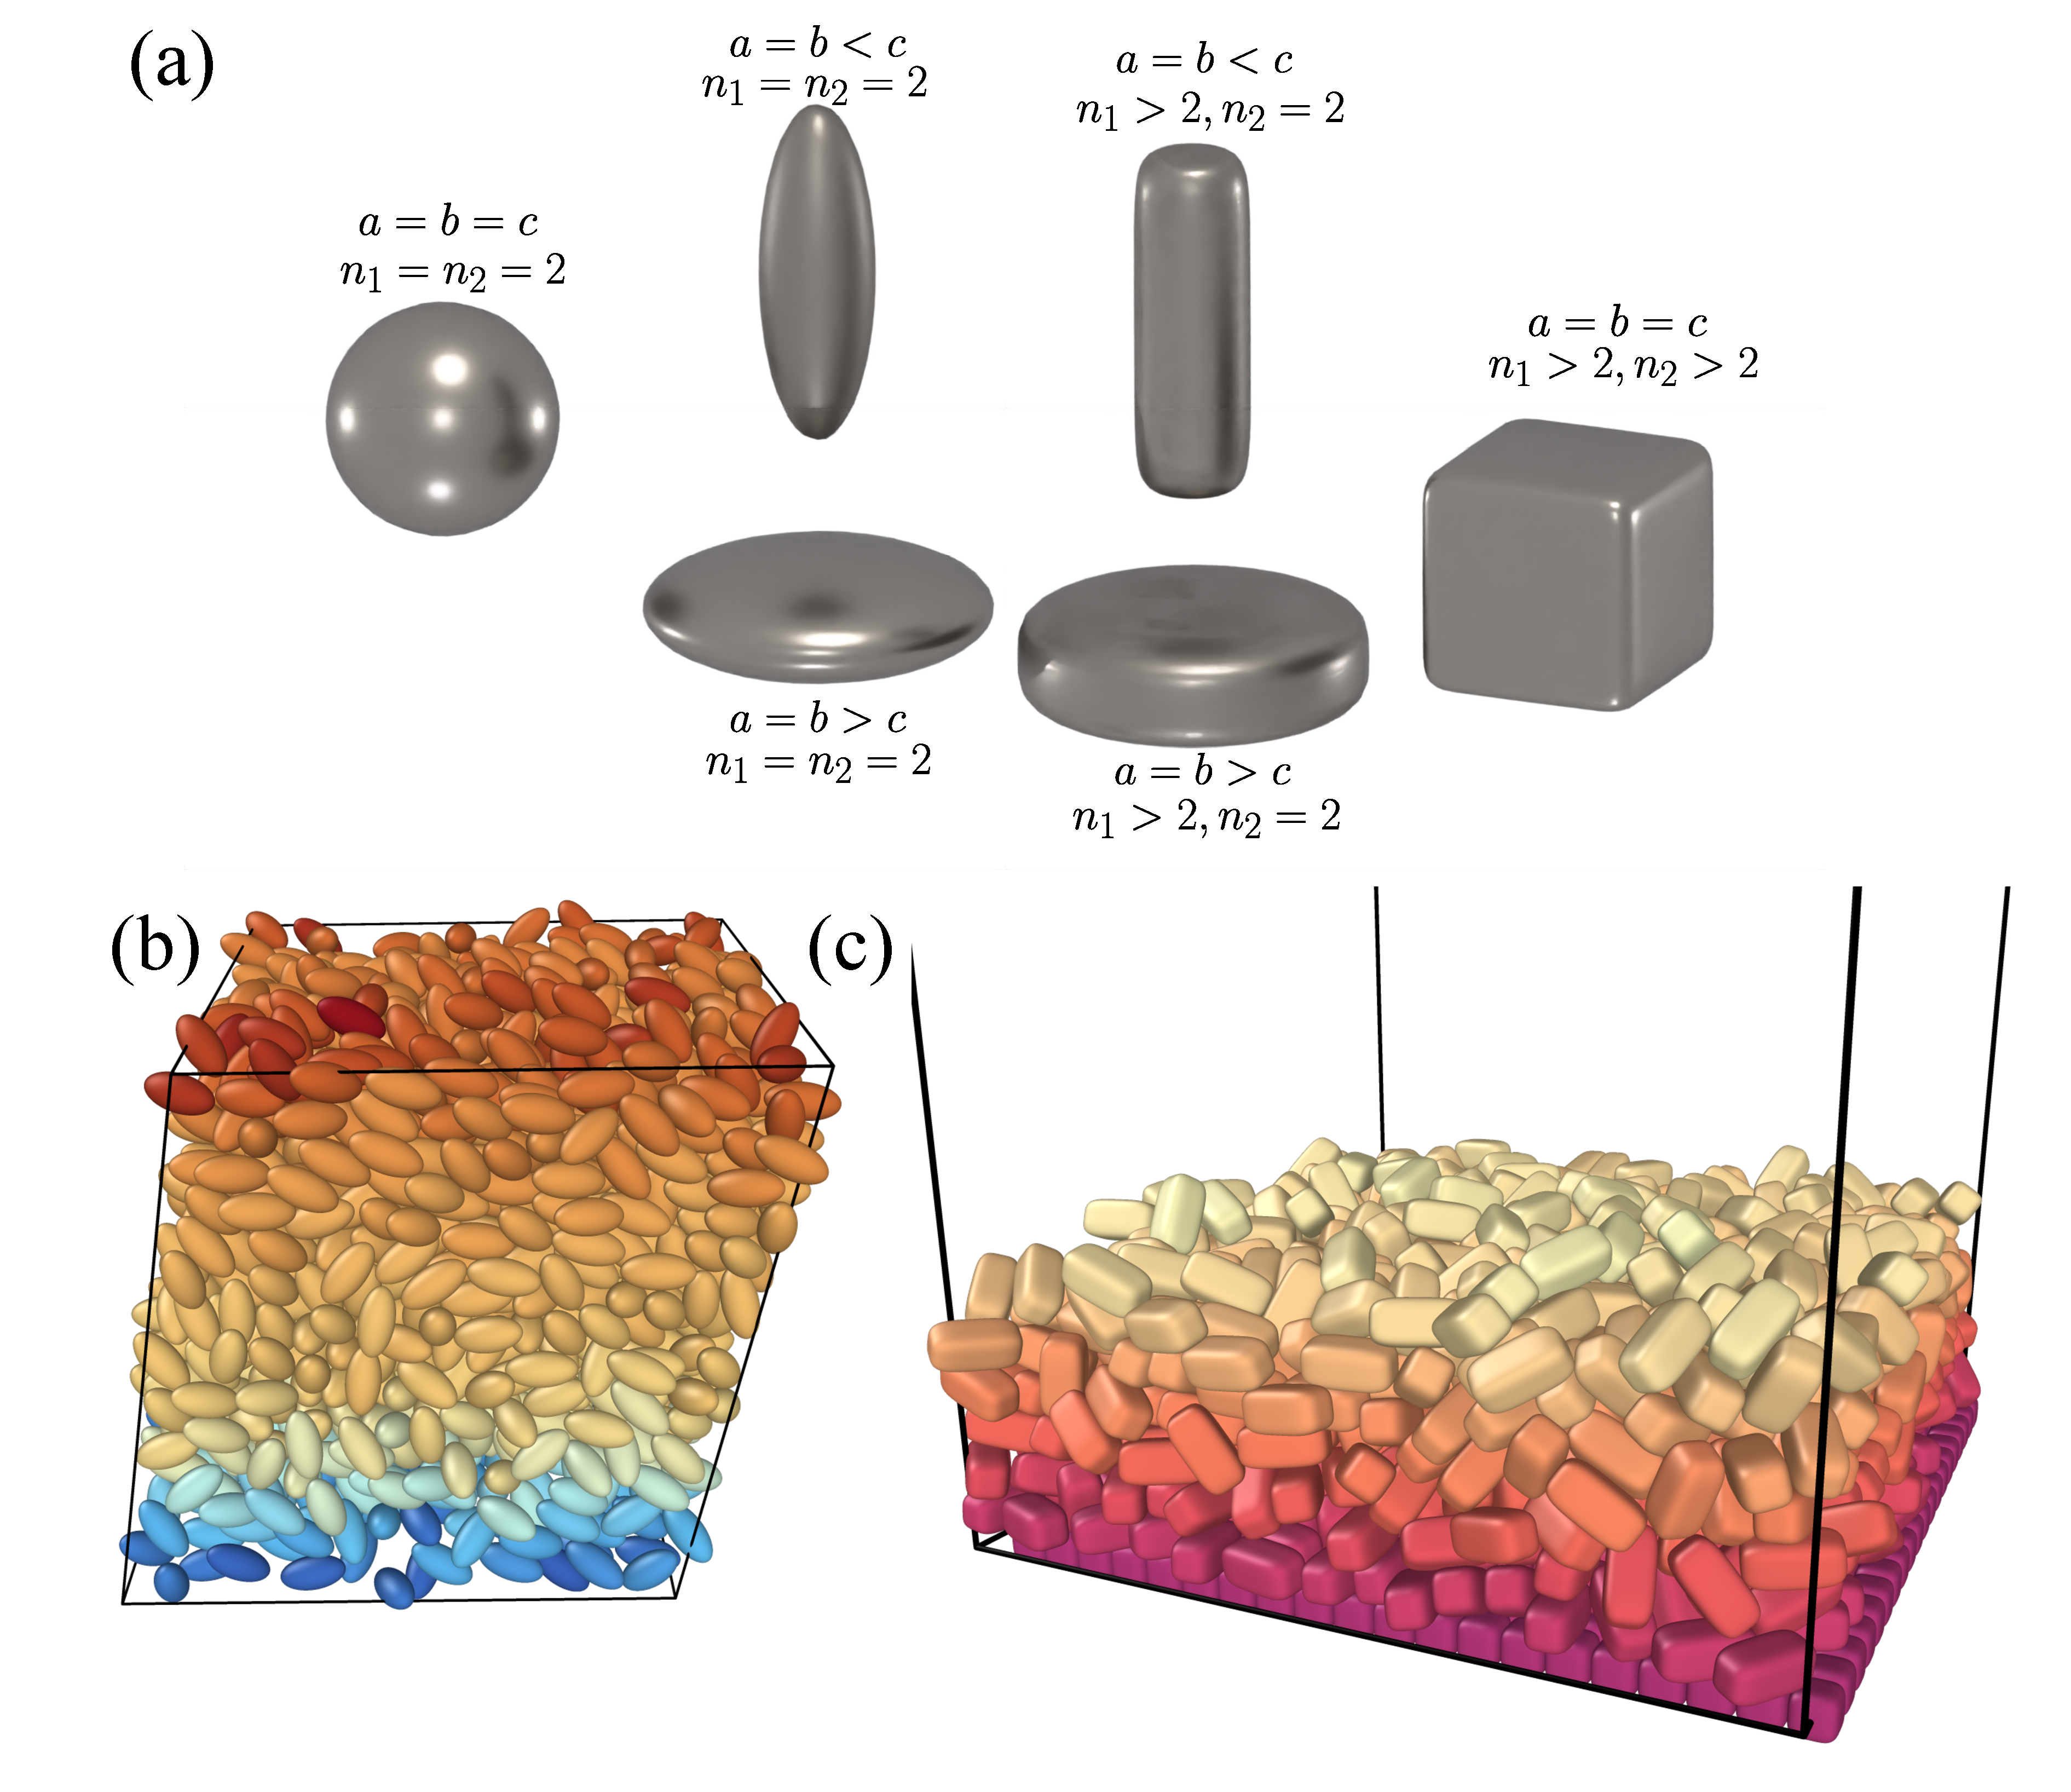
\includegraphics[width=.8\linewidth]{content/ch2/images/superellipsoidal_particles_lammps.pdf}
\caption{Panel (a) shows various particle morphologies generated simply by tuning the shape parameters, such as recovering spheres when $a=b=c$ and $n_1=n_2=2$ , or forming blocky cuboids when $a=b=c$ and $n_1>2, n_2>2$.
The bottom panels showcase practical system-level applications: (b) a rheological study of ellipsoidal particles undergoing continuous shear flow applied via the deform fix command, colored by their velocity in the flow direction; and (c)  a system of blocky superellipsoids settling under gravity, colored by their vertical position.}
\label{fig:superellipsoids}
\end{figure}
